\documentclass{standalone}
\usepackage{tikz}
\usetikzlibrary{patterns, positioning}


\begin{document}
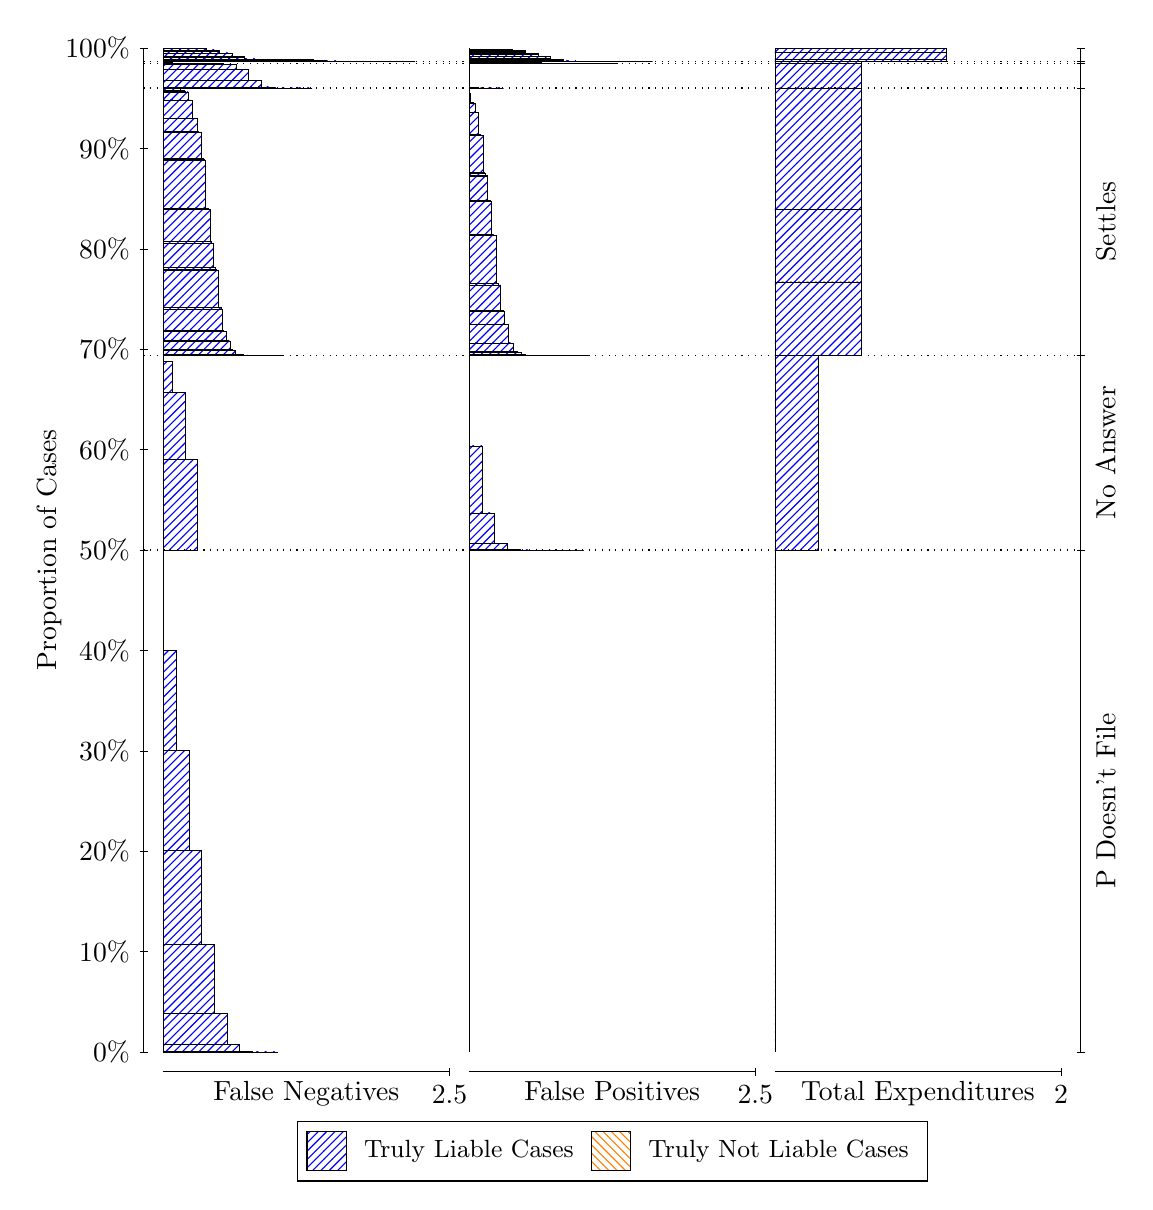
\begin{tikzpicture}
\draw[black, very thin] (1.5,1.75) -- (1.5,14.5);
\node[rotate=90, text=black, anchor=center] at (0.3, 8.125) {Proportion of Cases};
\draw[black, very thin] (1.45,1.75) -- (1.55,1.75);
\node[text=black, anchor=east] at (1.45, 1.75) {0\%};
\draw[black, very thin] (1.45,3.025) -- (1.55,3.025);
\node[text=black, anchor=east] at (1.45, 3.025) {10\%};
\draw[black, very thin] (1.45,4.3) -- (1.55,4.3);
\node[text=black, anchor=east] at (1.45, 4.3) {20\%};
\draw[black, very thin] (1.45,5.575) -- (1.55,5.575);
\node[text=black, anchor=east] at (1.45, 5.575) {30\%};
\draw[black, very thin] (1.45,6.85) -- (1.55,6.85);
\node[text=black, anchor=east] at (1.45, 6.85) {40\%};
\draw[black, very thin] (1.45,8.125) -- (1.55,8.125);
\node[text=black, anchor=east] at (1.45, 8.125) {50\%};
\draw[black, very thin] (1.45,9.4) -- (1.55,9.4);
\node[text=black, anchor=east] at (1.45, 9.4) {60\%};
\draw[black, very thin] (1.45,10.675) -- (1.55,10.675);
\node[text=black, anchor=east] at (1.45, 10.675) {70\%};
\draw[black, very thin] (1.45,11.95) -- (1.55,11.95);
\node[text=black, anchor=east] at (1.45, 11.95) {80\%};
\draw[black, very thin] (1.45,13.225) -- (1.55,13.225);
\node[text=black, anchor=east] at (1.45, 13.225) {90\%};
\draw[black, very thin] (1.45,14.5) -- (1.55,14.5);
\node[text=black, anchor=east] at (1.45, 14.5) {100\%};

\draw[black, very thin] (13.4,1.75) -- (13.4,14.5);
\draw[black, very thin] (13.35,1.75) -- (13.45,1.75);
\node[anchor=west] at (13.35, 1.75) {};
\draw[black, very thin] (13.35,8.125) -- (13.45,8.125);
\node[anchor=west] at (13.35, 8.125) {};
\draw[black, very thin] (13.35,10.6) -- (13.45,10.6);
\node[anchor=west] at (13.35, 10.6) {};
\draw[black, very thin] (13.35,13.993) -- (13.45,13.993);
\node[anchor=west] at (13.35, 13.993) {};
\draw[black, very thin] (13.35,14.3) -- (13.45,14.3);
\node[anchor=west] at (13.35, 14.3) {};
\draw[black, very thin] (13.35,14.331) -- (13.45,14.331);
\node[anchor=west] at (13.35, 14.331) {};
\draw[black, very thin] (13.35,14.5) -- (13.45,14.5);
\node[anchor=west] at (13.35, 14.5) {};

\draw[black, very thin, pattern color=blue, pattern=north east lines] (1.75,1.75) rectangle (3.2033,1.75);
\draw[black, very thin, pattern color=blue, pattern=north east lines] (1.75,1.75) rectangle (3.0419,1.7503);
\draw[black, very thin, pattern color=blue, pattern=north east lines] (1.75,1.7503) rectangle (2.8804,1.7583);
\draw[black, very thin, pattern color=blue, pattern=north east lines] (1.75,1.7583) rectangle (2.7189,1.8435);
\draw[black, very thin, pattern color=blue, pattern=north east lines] (1.75,1.8435) rectangle (2.5574,2.2369);
\draw[black, very thin, pattern color=blue, pattern=north east lines] (1.75,2.2369) rectangle (2.3959,3.1185);
\draw[black, very thin, pattern color=blue, pattern=north east lines] (1.75,3.1185) rectangle (2.2344,4.3083);
\draw[black, very thin, pattern color=blue, pattern=north east lines] (1.75,4.3083) rectangle (2.073,5.5753);
\draw[black, very thin, pattern color=blue, pattern=north east lines] (1.75,5.5753) rectangle (1.9115,6.85);
\draw[black, very thin, pattern color=orange, pattern=north west lines] (1.75,6.85) rectangle (1.75,6.85);
\draw[black, very thin, pattern color=blue, pattern=north east lines] (1.75,6.85) rectangle (1.75,8.125);
\draw[black, very thin, pattern color=blue, pattern=north east lines] (1.75,8.125) rectangle (2.186,9.2768);
\draw[black, very thin, pattern color=blue, pattern=north east lines] (1.75,9.2768) rectangle (2.0245,10.13);
\draw[black, very thin, pattern color=blue, pattern=north east lines] (1.75,10.13) rectangle (1.863,10.516);
\draw[black, very thin, pattern color=orange, pattern=north west lines] (1.75,10.516) rectangle (1.75,10.516);
\draw[black, very thin, pattern color=blue, pattern=north east lines] (1.75,10.516) rectangle (1.75,10.6);
\draw[black, very thin, pattern color=blue, pattern=north east lines] (1.75,10.6) rectangle (3.276,10.6);
\draw[black, very thin, pattern color=blue, pattern=north east lines] (1.75,10.6) rectangle (3.2033,10.6);
\draw[black, very thin, pattern color=blue, pattern=north east lines] (1.75,10.6) rectangle (3.1307,10.6);
\draw[black, very thin, pattern color=blue, pattern=north east lines] (1.75,10.6) rectangle (3.1145,10.6);
\draw[black, very thin, pattern color=blue, pattern=north east lines] (1.75,10.6) rectangle (3.058,10.6);
\draw[black, very thin, pattern color=blue, pattern=north east lines] (1.75,10.6) rectangle (3.0419,10.6);
\draw[black, very thin, pattern color=blue, pattern=north east lines] (1.75,10.6) rectangle (2.9853,10.6);
\draw[black, very thin, pattern color=blue, pattern=north east lines] (1.75,10.6) rectangle (2.9692,10.6);
\draw[black, very thin, pattern color=blue, pattern=north east lines] (1.75,10.6) rectangle (2.953,10.6);
\draw[black, very thin, pattern color=blue, pattern=north east lines] (1.75,10.6) rectangle (2.9127,10.6);
\draw[black, very thin, pattern color=blue, pattern=north east lines] (1.75,10.6) rectangle (2.8965,10.6);
\draw[black, very thin, pattern color=blue, pattern=north east lines] (1.75,10.6) rectangle (2.8804,10.6);
\draw[black, very thin, pattern color=blue, pattern=north east lines] (1.75,10.6) rectangle (2.84,10.6);
\draw[black, very thin, pattern color=blue, pattern=north east lines] (1.75,10.6) rectangle (2.8239,10.603);
\draw[black, very thin, pattern color=blue, pattern=north east lines] (1.75,10.603) rectangle (2.8077,10.603);
\draw[black, very thin, pattern color=blue, pattern=north east lines] (1.75,10.603) rectangle (2.7916,10.603);
\draw[black, very thin, pattern color=blue, pattern=north east lines] (1.75,10.603) rectangle (2.7673,10.612);
\draw[black, very thin, pattern color=blue, pattern=north east lines] (1.75,10.612) rectangle (2.7512,10.612);
\draw[black, very thin, pattern color=blue, pattern=north east lines] (1.75,10.612) rectangle (2.735,10.613);
\draw[black, very thin, pattern color=blue, pattern=north east lines] (1.75,10.613) rectangle (2.7189,10.613);
\draw[black, very thin, pattern color=blue, pattern=north east lines] (1.75,10.613) rectangle (2.6785,10.614);
\draw[black, very thin, pattern color=blue, pattern=north east lines] (1.75,10.614) rectangle (2.6624,10.662);
\draw[black, very thin, pattern color=blue, pattern=north east lines] (1.75,10.662) rectangle (2.6462,10.667);
\draw[black, very thin, pattern color=blue, pattern=north east lines] (1.75,10.667) rectangle (2.6301,10.669);
\draw[black, very thin, pattern color=blue, pattern=north east lines] (1.75,10.669) rectangle (2.6059,10.778);
\draw[black, very thin, pattern color=blue, pattern=north east lines] (1.75,10.778) rectangle (2.5897,10.781);
\draw[black, very thin, pattern color=blue, pattern=north east lines] (1.75,10.781) rectangle (2.5736,10.791);
\draw[black, very thin, pattern color=blue, pattern=north east lines] (1.75,10.791) rectangle (2.5574,10.793);
\draw[black, very thin, pattern color=blue, pattern=north east lines] (1.75,10.793) rectangle (2.5493,10.907);
\draw[black, very thin, pattern color=blue, pattern=north east lines] (1.75,10.907) rectangle (2.517,10.913);
\draw[black, very thin, pattern color=blue, pattern=north east lines] (1.75,10.913) rectangle (2.5009,11.185);
\draw[black, very thin, pattern color=blue, pattern=north east lines] (1.75,11.185) rectangle (2.4847,11.204);
\draw[black, very thin, pattern color=blue, pattern=north east lines] (1.75,11.204) rectangle (2.4686,11.208);
\draw[black, very thin, pattern color=blue, pattern=north east lines] (1.75,11.208) rectangle (2.4444,11.673);
\draw[black, very thin, pattern color=blue, pattern=north east lines] (1.75,11.673) rectangle (2.4282,11.685);
\draw[black, very thin, pattern color=blue, pattern=north east lines] (1.75,11.685) rectangle (2.4121,11.716);
\draw[black, very thin, pattern color=blue, pattern=north east lines] (1.75,11.716) rectangle (2.3959,11.718);
\draw[black, very thin, pattern color=blue, pattern=north east lines] (1.75,11.718) rectangle (2.3879,12.021);
\draw[black, very thin, pattern color=blue, pattern=north east lines] (1.75,12.021) rectangle (2.3556,12.044);
\draw[black, very thin, pattern color=blue, pattern=north east lines] (1.75,12.044) rectangle (2.3394,12.455);
\draw[black, very thin, pattern color=blue, pattern=north east lines] (1.75,12.455) rectangle (2.3233,12.468);
\draw[black, very thin, pattern color=blue, pattern=north east lines] (1.75,12.468) rectangle (2.3071,12.469);
\draw[black, very thin, pattern color=blue, pattern=north east lines] (1.75,12.469) rectangle (2.2829,13.076);
\draw[black, very thin, pattern color=blue, pattern=north east lines] (1.75,13.076) rectangle (2.2667,13.085);
\draw[black, very thin, pattern color=blue, pattern=north east lines] (1.75,13.085) rectangle (2.2506,13.103);
\draw[black, very thin, pattern color=blue, pattern=north east lines] (1.75,13.103) rectangle (2.2344,13.103);
\draw[black, very thin, pattern color=blue, pattern=north east lines] (1.75,13.103) rectangle (2.2264,13.425);
\draw[black, very thin, pattern color=blue, pattern=north east lines] (1.75,13.425) rectangle (2.1941,13.443);
\draw[black, very thin, pattern color=blue, pattern=north east lines] (1.75,13.443) rectangle (2.1779,13.605);
\draw[black, very thin, pattern color=blue, pattern=north east lines] (1.75,13.605) rectangle (2.1618,13.607);
\draw[black, very thin, pattern color=blue, pattern=north east lines] (1.75,13.607) rectangle (2.1456,13.607);
\draw[black, very thin, pattern color=blue, pattern=north east lines] (1.75,13.607) rectangle (2.1214,13.839);
\draw[black, very thin, pattern color=blue, pattern=north east lines] (1.75,13.839) rectangle (2.1053,13.84);
\draw[black, very thin, pattern color=blue, pattern=north east lines] (1.75,13.84) rectangle (2.0891,13.842);
\draw[black, very thin, pattern color=blue, pattern=north east lines] (1.75,13.842) rectangle (2.073,13.842);
\draw[black, very thin, pattern color=blue, pattern=north east lines] (1.75,13.842) rectangle (2.0649,13.944);
\draw[black, very thin, pattern color=blue, pattern=north east lines] (1.75,13.944) rectangle (2.0326,13.946);
\draw[black, very thin, pattern color=blue, pattern=north east lines] (1.75,13.946) rectangle (2.0164,13.961);
\draw[black, very thin, pattern color=blue, pattern=north east lines] (1.75,13.961) rectangle (2.0003,13.961);
\draw[black, very thin, pattern color=blue, pattern=north east lines] (1.75,13.961) rectangle (1.9841,13.961);
\draw[black, very thin, pattern color=blue, pattern=north east lines] (1.75,13.961) rectangle (1.9599,13.984);
\draw[black, very thin, pattern color=blue, pattern=north east lines] (1.75,13.984) rectangle (1.9438,13.984);
\draw[black, very thin, pattern color=blue, pattern=north east lines] (1.75,13.984) rectangle (1.9276,13.984);
\draw[black, very thin, pattern color=blue, pattern=north east lines] (1.75,13.984) rectangle (1.9115,13.984);
\draw[black, very thin, pattern color=blue, pattern=north east lines] (1.75,13.984) rectangle (1.9034,13.992);
\draw[black, very thin, pattern color=blue, pattern=north east lines] (1.75,13.992) rectangle (1.8711,13.992);
\draw[black, very thin, pattern color=blue, pattern=north east lines] (1.75,13.992) rectangle (1.855,13.993);
\draw[black, very thin, pattern color=blue, pattern=north east lines] (1.75,13.993) rectangle (1.8388,13.993);
\draw[black, very thin, pattern color=blue, pattern=north east lines] (1.75,13.993) rectangle (1.8227,13.993);
\draw[black, very thin, pattern color=blue, pattern=north east lines] (1.75,13.993) rectangle (1.7984,13.993);
\draw[black, very thin, pattern color=blue, pattern=north east lines] (1.75,13.993) rectangle (1.7823,13.993);
\draw[black, very thin, pattern color=blue, pattern=north east lines] (1.75,13.993) rectangle (1.7661,13.993);
\draw[black, very thin, pattern color=orange, pattern=north west lines] (1.75,13.993) rectangle (1.75,13.993);
\draw[black, very thin, pattern color=blue, pattern=north east lines] (1.75,13.993) rectangle (1.75,13.993);
\draw[black, very thin, pattern color=blue, pattern=north east lines] (1.75,13.993) rectangle (3.6393,13.993);
\draw[black, very thin, pattern color=blue, pattern=north east lines] (1.75,13.993) rectangle (3.4779,13.993);
\draw[black, very thin, pattern color=blue, pattern=north east lines] (1.75,13.993) rectangle (3.3164,13.994);
\draw[black, very thin, pattern color=blue, pattern=north east lines] (1.75,13.994) rectangle (3.1549,14.006);
\draw[black, very thin, pattern color=blue, pattern=north east lines] (1.75,14.006) rectangle (2.9934,14.091);
\draw[black, very thin, pattern color=blue, pattern=north east lines] (1.75,14.091) rectangle (2.8319,14.232);
\draw[black, very thin, pattern color=blue, pattern=north east lines] (1.75,14.232) rectangle (2.6704,14.293);
\draw[black, very thin, pattern color=blue, pattern=north east lines] (1.75,14.293) rectangle (2.509,14.3);
\draw[black, very thin, pattern color=blue, pattern=north east lines] (1.75,14.3) rectangle (2.3475,14.3);
\draw[black, very thin, pattern color=blue, pattern=north east lines] (1.75,14.3) rectangle (2.186,14.3);
\draw[black, very thin, pattern color=orange, pattern=north west lines] (1.75,14.3) rectangle (1.75,14.3);
\draw[black, very thin, pattern color=blue, pattern=north east lines] (1.75,14.3) rectangle (2.186,14.3);
\draw[black, very thin, pattern color=blue, pattern=north east lines] (1.75,14.3) rectangle (2.0245,14.302);
\draw[black, very thin, pattern color=blue, pattern=north east lines] (1.75,14.302) rectangle (1.863,14.313);
\draw[black, very thin, pattern color=orange, pattern=north west lines] (1.75,14.313) rectangle (1.75,14.313);
\draw[black, very thin, pattern color=blue, pattern=north east lines] (1.75,14.313) rectangle (1.75,14.331);
\draw[black, very thin, pattern color=blue, pattern=north east lines] (1.75,14.331) rectangle (4.9473,14.331);
\draw[black, very thin, pattern color=blue, pattern=north east lines] (1.75,14.331) rectangle (4.7859,14.331);
\draw[black, very thin, pattern color=blue, pattern=north east lines] (1.75,14.331) rectangle (4.6244,14.331);
\draw[black, very thin, pattern color=blue, pattern=north east lines] (1.75,14.331) rectangle (4.6244,14.331);
\draw[black, very thin, pattern color=blue, pattern=north east lines] (1.75,14.331) rectangle (4.4629,14.331);
\draw[black, very thin, pattern color=blue, pattern=north east lines] (1.75,14.331) rectangle (4.3014,14.331);
\draw[black, very thin, pattern color=blue, pattern=north east lines] (1.75,14.331) rectangle (4.1399,14.332);
\draw[black, very thin, pattern color=blue, pattern=north east lines] (1.75,14.332) rectangle (3.9784,14.338);
\draw[black, very thin, pattern color=blue, pattern=north east lines] (1.75,14.338) rectangle (3.817,14.341);
\draw[black, very thin, pattern color=blue, pattern=north east lines] (1.75,14.341) rectangle (3.817,14.347);
\draw[black, very thin, pattern color=blue, pattern=north east lines] (1.75,14.347) rectangle (3.7524,14.347);
\draw[black, very thin, pattern color=blue, pattern=north east lines] (1.75,14.347) rectangle (3.6555,14.351);
\draw[black, very thin, pattern color=blue, pattern=north east lines] (1.75,14.351) rectangle (3.6555,14.351);
\draw[black, very thin, pattern color=blue, pattern=north east lines] (1.75,14.351) rectangle (3.5909,14.351);
\draw[black, very thin, pattern color=blue, pattern=north east lines] (1.75,14.351) rectangle (3.494,14.351);
\draw[black, very thin, pattern color=blue, pattern=north east lines] (1.75,14.351) rectangle (3.4294,14.351);
\draw[black, very thin, pattern color=blue, pattern=north east lines] (1.75,14.351) rectangle (3.3325,14.351);
\draw[black, very thin, pattern color=blue, pattern=north east lines] (1.75,14.351) rectangle (3.3325,14.351);
\draw[black, very thin, pattern color=blue, pattern=north east lines] (1.75,14.351) rectangle (3.2679,14.351);
\draw[black, very thin, pattern color=blue, pattern=north east lines] (1.75,14.351) rectangle (3.2679,14.351);
\draw[black, very thin, pattern color=blue, pattern=north east lines] (1.75,14.351) rectangle (3.171,14.351);
\draw[black, very thin, pattern color=blue, pattern=north east lines] (1.75,14.351) rectangle (3.171,14.351);
\draw[black, very thin, pattern color=blue, pattern=north east lines] (1.75,14.351) rectangle (3.1064,14.352);
\draw[black, very thin, pattern color=blue, pattern=north east lines] (1.75,14.352) rectangle (3.1064,14.352);
\draw[black, very thin, pattern color=blue, pattern=north east lines] (1.75,14.352) rectangle (3.0096,14.352);
\draw[black, very thin, pattern color=blue, pattern=north east lines] (1.75,14.352) rectangle (2.945,14.362);
\draw[black, very thin, pattern color=blue, pattern=north east lines] (1.75,14.362) rectangle (2.8481,14.362);
\draw[black, very thin, pattern color=blue, pattern=north east lines] (1.75,14.362) rectangle (2.7835,14.377);
\draw[black, very thin, pattern color=blue, pattern=north east lines] (1.75,14.377) rectangle (2.7835,14.395);
\draw[black, very thin, pattern color=blue, pattern=north east lines] (1.75,14.395) rectangle (2.622,14.439);
\draw[black, very thin, pattern color=blue, pattern=north east lines] (1.75,14.439) rectangle (2.4605,14.457);
\draw[black, very thin, pattern color=blue, pattern=north east lines] (1.75,14.457) rectangle (2.4605,14.457);
\draw[black, very thin, pattern color=blue, pattern=north east lines] (1.75,14.457) rectangle (2.4605,14.475);
\draw[black, very thin, pattern color=blue, pattern=north east lines] (1.75,14.475) rectangle (2.299,14.493);
\draw[black, very thin, pattern color=blue, pattern=north east lines] (1.75,14.493) rectangle (2.299,14.494);
\draw[black, very thin, pattern color=blue, pattern=north east lines] (1.75,14.494) rectangle (2.1376,14.496);
\draw[black, very thin, pattern color=blue, pattern=north east lines] (1.75,14.496) rectangle (2.1376,14.496);
\draw[black, very thin, pattern color=blue, pattern=north east lines] (1.75,14.496) rectangle (2.1376,14.499);
\draw[black, very thin, pattern color=blue, pattern=north east lines] (1.75,14.499) rectangle (1.9761,14.5);
\draw[black, very thin, pattern color=blue, pattern=north east lines] (1.75,14.5) rectangle (1.9761,14.5);
\draw[black, very thin, pattern color=blue, pattern=north east lines] (1.75,14.5) rectangle (1.8146,14.5);
\draw[black, very thin, pattern color=blue, pattern=north east lines] (1.75,14.5) rectangle (1.8146,14.5);
\draw[black, very thin, pattern color=orange, pattern=north west lines] (1.75,14.5) rectangle (1.75,14.5);
\draw[black, very thin, pattern color=blue, pattern=north east lines] (1.75,14.5) rectangle (1.75,14.5);
\draw[black, very thin, pattern color=orange, pattern=north west lines] (5.6333,1.75) rectangle (5.6333,1.75);
\draw[black, very thin, pattern color=blue, pattern=north east lines] (5.6333,1.75) rectangle (5.6333,8.125);
\draw[black, very thin, pattern color=orange, pattern=north west lines] (5.6333,8.125) rectangle (7.0867,8.125);
\draw[black, very thin, pattern color=blue, pattern=north east lines] (5.6333,8.125) rectangle (7.0867,8.125);
\draw[black, very thin, pattern color=blue, pattern=north east lines] (5.6333,8.125) rectangle (6.9252,8.125);
\draw[black, very thin, pattern color=blue, pattern=north east lines] (5.6333,8.125) rectangle (6.7637,8.125);
\draw[black, very thin, pattern color=blue, pattern=north east lines] (5.6333,8.125) rectangle (6.6022,8.125);
\draw[black, very thin, pattern color=blue, pattern=north east lines] (5.6333,8.125) rectangle (6.4407,8.1251);
\draw[black, very thin, pattern color=blue, pattern=north east lines] (5.6333,8.1251) rectangle (6.2793,8.1306);
\draw[black, very thin, pattern color=blue, pattern=north east lines] (5.6333,8.1306) rectangle (6.1178,8.2098);
\draw[black, very thin, pattern color=blue, pattern=north east lines] (5.6333,8.2098) rectangle (5.9563,8.5952);
\draw[black, very thin, pattern color=blue, pattern=north east lines] (5.6333,8.5952) rectangle (5.7948,9.4485);
\draw[black, very thin, pattern color=blue, pattern=north east lines] (5.6333,9.4485) rectangle (5.6333,10.6);
\draw[black, very thin, pattern color=orange, pattern=north west lines] (5.6333,10.6) rectangle (7.1593,10.6);
\draw[black, very thin, pattern color=blue, pattern=north east lines] (5.6333,10.6) rectangle (7.1593,10.6);
\draw[black, very thin, pattern color=blue, pattern=north east lines] (5.6333,10.6) rectangle (6.9979,10.6);
\draw[black, very thin, pattern color=orange, pattern=north west lines] (5.6333,10.6) rectangle (6.9413,10.6);
\draw[black, very thin, pattern color=blue, pattern=north east lines] (5.6333,10.6) rectangle (6.9413,10.6);
\draw[black, very thin, pattern color=orange, pattern=north west lines] (5.6333,10.6) rectangle (6.8687,10.6);
\draw[black, very thin, pattern color=blue, pattern=north east lines] (5.6333,10.6) rectangle (6.8687,10.6);
\draw[black, very thin, pattern color=blue, pattern=north east lines] (5.6333,10.6) rectangle (6.8364,10.6);
\draw[black, very thin, pattern color=orange, pattern=north west lines] (5.6333,10.6) rectangle (6.796,10.6);
\draw[black, very thin, pattern color=blue, pattern=north east lines] (5.6333,10.6) rectangle (6.796,10.6);
\draw[black, very thin, pattern color=blue, pattern=north east lines] (5.6333,10.6) rectangle (6.7799,10.6);
\draw[black, very thin, pattern color=orange, pattern=north west lines] (5.6333,10.6) rectangle (6.7233,10.6);
\draw[black, very thin, pattern color=blue, pattern=north east lines] (5.6333,10.6) rectangle (6.7233,10.6);
\draw[black, very thin, pattern color=blue, pattern=north east lines] (5.6333,10.6) rectangle (6.7072,10.6);
\draw[black, very thin, pattern color=blue, pattern=north east lines] (5.6333,10.6) rectangle (6.6749,10.6);
\draw[black, very thin, pattern color=orange, pattern=north west lines] (5.6333,10.6) rectangle (6.6507,10.6);
\draw[black, very thin, pattern color=blue, pattern=north east lines] (5.6333,10.6) rectangle (6.6507,10.6);
\draw[black, very thin, pattern color=blue, pattern=north east lines] (5.6333,10.6) rectangle (6.6345,10.6);
\draw[black, very thin, pattern color=blue, pattern=north east lines] (5.6333,10.6) rectangle (6.6184,10.6);
\draw[black, very thin, pattern color=orange, pattern=north west lines] (5.6333,10.6) rectangle (6.578,10.6);
\draw[black, very thin, pattern color=blue, pattern=north east lines] (5.6333,10.6) rectangle (6.578,10.6);
\draw[black, very thin, pattern color=blue, pattern=north east lines] (5.6333,10.6) rectangle (6.5619,10.6);
\draw[black, very thin, pattern color=blue, pattern=north east lines] (5.6333,10.6) rectangle (6.5457,10.6);
\draw[black, very thin, pattern color=blue, pattern=north east lines] (5.6333,10.6) rectangle (6.5134,10.6);
\draw[black, very thin, pattern color=orange, pattern=north west lines] (5.6333,10.6) rectangle (6.5053,10.6);
\draw[black, very thin, pattern color=blue, pattern=north east lines] (5.6333,10.6) rectangle (6.5053,10.6);
\draw[black, very thin, pattern color=blue, pattern=north east lines] (5.6333,10.6) rectangle (6.4892,10.6);
\draw[black, very thin, pattern color=blue, pattern=north east lines] (5.6333,10.6) rectangle (6.473,10.6);
\draw[black, very thin, pattern color=blue, pattern=north east lines] (5.6333,10.6) rectangle (6.4569,10.601);
\draw[black, very thin, pattern color=orange, pattern=north west lines] (5.6333,10.601) rectangle (6.4327,10.601);
\draw[black, very thin, pattern color=blue, pattern=north east lines] (5.6333,10.601) rectangle (6.4327,10.601);
\draw[black, very thin, pattern color=blue, pattern=north east lines] (5.6333,10.601) rectangle (6.4165,10.601);
\draw[black, very thin, pattern color=blue, pattern=north east lines] (5.6333,10.601) rectangle (6.4004,10.601);
\draw[black, very thin, pattern color=blue, pattern=north east lines] (5.6333,10.601) rectangle (6.3842,10.601);
\draw[black, very thin, pattern color=blue, pattern=north east lines] (5.6333,10.601) rectangle (6.3519,10.61);
\draw[black, very thin, pattern color=blue, pattern=north east lines] (5.6333,10.61) rectangle (6.3439,10.61);
\draw[black, very thin, pattern color=blue, pattern=north east lines] (5.6333,10.61) rectangle (6.3277,10.61);
\draw[black, very thin, pattern color=blue, pattern=north east lines] (5.6333,10.61) rectangle (6.3116,10.61);
\draw[black, very thin, pattern color=blue, pattern=north east lines] (5.6333,10.61) rectangle (6.2954,10.632);
\draw[black, very thin, pattern color=blue, pattern=north east lines] (5.6333,10.632) rectangle (6.2712,10.632);
\draw[black, very thin, pattern color=blue, pattern=north east lines] (5.6333,10.632) rectangle (6.255,10.632);
\draw[black, very thin, pattern color=blue, pattern=north east lines] (5.6333,10.632) rectangle (6.2389,10.647);
\draw[black, very thin, pattern color=blue, pattern=north east lines] (5.6333,10.647) rectangle (6.2227,10.65);
\draw[black, very thin, pattern color=blue, pattern=north east lines] (5.6333,10.65) rectangle (6.1904,10.752);
\draw[black, very thin, pattern color=blue, pattern=north east lines] (5.6333,10.752) rectangle (6.1824,10.752);
\draw[black, very thin, pattern color=blue, pattern=north east lines] (5.6333,10.752) rectangle (6.1662,10.754);
\draw[black, very thin, pattern color=blue, pattern=north east lines] (5.6333,10.754) rectangle (6.1501,10.755);
\draw[black, very thin, pattern color=blue, pattern=north east lines] (5.6333,10.755) rectangle (6.1339,10.987);
\draw[black, very thin, pattern color=blue, pattern=north east lines] (5.6333,10.987) rectangle (6.1097,10.987);
\draw[black, very thin, pattern color=blue, pattern=north east lines] (5.6333,10.987) rectangle (6.0936,10.988);
\draw[black, very thin, pattern color=blue, pattern=north east lines] (5.6333,10.988) rectangle (6.0774,11.151);
\draw[black, very thin, pattern color=blue, pattern=north east lines] (5.6333,11.151) rectangle (6.0613,11.168);
\draw[black, very thin, pattern color=blue, pattern=north east lines] (5.6333,11.168) rectangle (6.029,11.491);
\draw[black, very thin, pattern color=blue, pattern=north east lines] (5.6333,11.491) rectangle (6.0209,11.491);
\draw[black, very thin, pattern color=blue, pattern=north east lines] (5.6333,11.491) rectangle (6.0047,11.509);
\draw[black, very thin, pattern color=blue, pattern=north east lines] (5.6333,11.509) rectangle (5.9886,11.518);
\draw[black, very thin, pattern color=blue, pattern=north east lines] (5.6333,11.518) rectangle (5.9724,12.124);
\draw[black, very thin, pattern color=blue, pattern=north east lines] (5.6333,12.124) rectangle (5.9482,12.126);
\draw[black, very thin, pattern color=blue, pattern=north east lines] (5.6333,12.126) rectangle (5.9321,12.138);
\draw[black, very thin, pattern color=blue, pattern=north east lines] (5.6333,12.138) rectangle (5.9159,12.549);
\draw[black, very thin, pattern color=blue, pattern=north east lines] (5.6333,12.549) rectangle (5.8998,12.572);
\draw[black, very thin, pattern color=blue, pattern=north east lines] (5.6333,12.572) rectangle (5.8675,12.876);
\draw[black, very thin, pattern color=blue, pattern=north east lines] (5.6333,12.876) rectangle (5.8594,12.878);
\draw[black, very thin, pattern color=blue, pattern=north east lines] (5.6333,12.878) rectangle (5.8433,12.909);
\draw[black, very thin, pattern color=blue, pattern=north east lines] (5.6333,12.909) rectangle (5.8271,12.92);
\draw[black, very thin, pattern color=blue, pattern=north east lines] (5.6333,12.92) rectangle (5.811,13.386);
\draw[black, very thin, pattern color=blue, pattern=north east lines] (5.6333,13.386) rectangle (5.7867,13.389);
\draw[black, very thin, pattern color=blue, pattern=north east lines] (5.6333,13.389) rectangle (5.7706,13.409);
\draw[black, very thin, pattern color=blue, pattern=north east lines] (5.6333,13.409) rectangle (5.7544,13.681);
\draw[black, very thin, pattern color=blue, pattern=north east lines] (5.6333,13.681) rectangle (5.7383,13.687);
\draw[black, very thin, pattern color=blue, pattern=north east lines] (5.6333,13.687) rectangle (5.706,13.8);
\draw[black, very thin, pattern color=blue, pattern=north east lines] (5.6333,13.8) rectangle (5.6979,13.802);
\draw[black, very thin, pattern color=blue, pattern=north east lines] (5.6333,13.802) rectangle (5.6818,13.812);
\draw[black, very thin, pattern color=blue, pattern=north east lines] (5.6333,13.812) rectangle (5.6656,13.815);
\draw[black, very thin, pattern color=blue, pattern=north east lines] (5.6333,13.815) rectangle (5.6495,13.924);
\draw[black, very thin, pattern color=blue, pattern=north east lines] (5.6333,13.924) rectangle (5.6333,13.993);
\draw[black, very thin, pattern color=orange, pattern=north west lines] (5.6333,13.993) rectangle (6.0693,13.993);
\draw[black, very thin, pattern color=blue, pattern=north east lines] (5.6333,13.993) rectangle (6.0693,13.993);
\draw[black, very thin, pattern color=blue, pattern=north east lines] (5.6333,13.993) rectangle (5.9079,13.993);
\draw[black, very thin, pattern color=blue, pattern=north east lines] (5.6333,13.993) rectangle (5.7464,14.001);
\draw[black, very thin, pattern color=blue, pattern=north east lines] (5.6333,14.001) rectangle (5.6333,14.3);
\draw[black, very thin, pattern color=orange, pattern=north west lines] (5.6333,14.3) rectangle (7.5227,14.3);
\draw[black, very thin, pattern color=blue, pattern=north east lines] (5.6333,14.3) rectangle (7.5227,14.3);
\draw[black, very thin, pattern color=blue, pattern=north east lines] (5.6333,14.3) rectangle (7.3612,14.3);
\draw[black, very thin, pattern color=blue, pattern=north east lines] (5.6333,14.3) rectangle (7.1997,14.3);
\draw[black, very thin, pattern color=blue, pattern=north east lines] (5.6333,14.3) rectangle (7.0382,14.3);
\draw[black, very thin, pattern color=blue, pattern=north east lines] (5.6333,14.3) rectangle (6.8767,14.3);
\draw[black, very thin, pattern color=blue, pattern=north east lines] (5.6333,14.3) rectangle (6.7153,14.304);
\draw[black, very thin, pattern color=blue, pattern=north east lines] (5.6333,14.304) rectangle (6.5538,14.318);
\draw[black, very thin, pattern color=blue, pattern=north east lines] (5.6333,14.318) rectangle (6.3923,14.328);
\draw[black, very thin, pattern color=blue, pattern=north east lines] (5.6333,14.328) rectangle (6.2308,14.331);
\draw[black, very thin, pattern color=blue, pattern=north east lines] (5.6333,14.331) rectangle (6.0693,14.331);
\draw[black, very thin, pattern color=orange, pattern=north west lines] (5.6333,14.331) rectangle (7.9587,14.331);
\draw[black, very thin, pattern color=blue, pattern=north east lines] (5.6333,14.331) rectangle (7.9587,14.331);
\draw[black, very thin, pattern color=orange, pattern=north west lines] (5.6333,14.331) rectangle (7.7972,14.331);
\draw[black, very thin, pattern color=blue, pattern=north east lines] (5.6333,14.331) rectangle (7.7972,14.331);
\draw[black, very thin, pattern color=orange, pattern=north west lines] (5.6333,14.331) rectangle (7.6357,14.331);
\draw[black, very thin, pattern color=blue, pattern=north east lines] (5.6333,14.331) rectangle (7.6357,14.331);
\draw[black, very thin, pattern color=blue, pattern=north east lines] (5.6333,14.331) rectangle (7.4742,14.331);
\draw[black, very thin, pattern color=orange, pattern=north west lines] (5.6333,14.331) rectangle (7.4742,14.331);
\draw[black, very thin, pattern color=blue, pattern=north east lines] (5.6333,14.331) rectangle (7.4742,14.331);
\draw[black, very thin, pattern color=blue, pattern=north east lines] (5.6333,14.331) rectangle (7.3127,14.331);
\draw[black, very thin, pattern color=orange, pattern=north west lines] (5.6333,14.331) rectangle (7.3127,14.331);
\draw[black, very thin, pattern color=blue, pattern=north east lines] (5.6333,14.331) rectangle (7.3127,14.331);
\draw[black, very thin, pattern color=blue, pattern=north east lines] (5.6333,14.331) rectangle (7.1513,14.331);
\draw[black, very thin, pattern color=orange, pattern=north west lines] (5.6333,14.331) rectangle (7.1513,14.331);
\draw[black, very thin, pattern color=blue, pattern=north east lines] (5.6333,14.331) rectangle (7.1513,14.331);
\draw[black, very thin, pattern color=blue, pattern=north east lines] (5.6333,14.331) rectangle (6.9898,14.333);
\draw[black, very thin, pattern color=orange, pattern=north west lines] (5.6333,14.333) rectangle (6.9898,14.333);
\draw[black, very thin, pattern color=blue, pattern=north east lines] (5.6333,14.333) rectangle (6.9898,14.337);
\draw[black, very thin, pattern color=blue, pattern=north east lines] (5.6333,14.337) rectangle (6.9898,14.337);
\draw[black, very thin, pattern color=blue, pattern=north east lines] (5.6333,14.337) rectangle (6.9898,14.337);
\draw[black, very thin, pattern color=blue, pattern=north east lines] (5.6333,14.337) rectangle (6.8283,14.346);
\draw[black, very thin, pattern color=orange, pattern=north west lines] (5.6333,14.346) rectangle (6.8283,14.346);
\draw[black, very thin, pattern color=blue, pattern=north east lines] (5.6333,14.346) rectangle (6.8283,14.355);
\draw[black, very thin, pattern color=blue, pattern=north east lines] (5.6333,14.355) rectangle (6.8283,14.355);
\draw[black, very thin, pattern color=blue, pattern=north east lines] (5.6333,14.355) rectangle (6.6668,14.356);
\draw[black, very thin, pattern color=blue, pattern=north east lines] (5.6333,14.356) rectangle (6.6668,14.373);
\draw[black, very thin, pattern color=blue, pattern=north east lines] (5.6333,14.373) rectangle (6.6668,14.391);
\draw[black, very thin, pattern color=blue, pattern=north east lines] (5.6333,14.391) rectangle (6.5053,14.394);
\draw[black, very thin, pattern color=blue, pattern=north east lines] (5.6333,14.394) rectangle (6.5053,14.415);
\draw[black, very thin, pattern color=blue, pattern=north east lines] (5.6333,14.415) rectangle (6.5053,14.436);
\draw[black, very thin, pattern color=blue, pattern=north east lines] (5.6333,14.436) rectangle (6.3439,14.442);
\draw[black, very thin, pattern color=blue, pattern=north east lines] (5.6333,14.442) rectangle (6.3439,14.442);
\draw[black, very thin, pattern color=blue, pattern=north east lines] (5.6333,14.442) rectangle (6.3439,14.459);
\draw[black, very thin, pattern color=blue, pattern=north east lines] (5.6333,14.459) rectangle (6.3439,14.468);
\draw[black, very thin, pattern color=orange, pattern=north west lines] (5.6333,14.468) rectangle (6.2793,14.468);
\draw[black, very thin, pattern color=blue, pattern=north east lines] (5.6333,14.468) rectangle (6.2793,14.468);
\draw[black, very thin, pattern color=blue, pattern=north east lines] (5.6333,14.468) rectangle (6.1824,14.473);
\draw[black, very thin, pattern color=blue, pattern=north east lines] (5.6333,14.473) rectangle (6.1824,14.478);
\draw[black, very thin, pattern color=orange, pattern=north west lines] (5.6333,14.478) rectangle (6.1178,14.478);
\draw[black, very thin, pattern color=blue, pattern=north east lines] (5.6333,14.478) rectangle (6.1178,14.478);
\draw[black, very thin, pattern color=blue, pattern=north east lines] (5.6333,14.478) rectangle (6.0209,14.479);
\draw[black, very thin, pattern color=blue, pattern=north east lines] (5.6333,14.479) rectangle (6.0209,14.479);
\draw[black, very thin, pattern color=blue, pattern=north east lines] (5.6333,14.479) rectangle (6.0209,14.479);
\draw[black, very thin, pattern color=orange, pattern=north west lines] (5.6333,14.479) rectangle (5.9563,14.479);
\draw[black, very thin, pattern color=blue, pattern=north east lines] (5.6333,14.479) rectangle (5.9563,14.479);
\draw[black, very thin, pattern color=blue, pattern=north east lines] (5.6333,14.479) rectangle (5.8594,14.479);
\draw[black, very thin, pattern color=blue, pattern=north east lines] (5.6333,14.479) rectangle (5.8594,14.479);
\draw[black, very thin, pattern color=orange, pattern=north west lines] (5.6333,14.479) rectangle (5.7948,14.479);
\draw[black, very thin, pattern color=blue, pattern=north east lines] (5.6333,14.479) rectangle (5.7948,14.479);
\draw[black, very thin, pattern color=blue, pattern=north east lines] (5.6333,14.479) rectangle (5.6979,14.479);
\draw[black, very thin, pattern color=blue, pattern=north east lines] (5.6333,14.479) rectangle (5.6979,14.479);
\draw[black, very thin, pattern color=blue, pattern=north east lines] (5.6333,14.479) rectangle (5.6979,14.479);
\draw[black, very thin, pattern color=orange, pattern=north west lines] (5.6333,14.479) rectangle (5.6333,14.479);
\draw[black, very thin, pattern color=blue, pattern=north east lines] (5.6333,14.479) rectangle (5.6333,14.5);
\draw[black, very thin, pattern color=orange, pattern=north west lines] (9.5167,1.75) rectangle (9.5167,1.75);
\draw[black, very thin, pattern color=blue, pattern=north east lines] (9.5167,1.75) rectangle (9.5167,8.125);
\draw[black, very thin, pattern color=orange, pattern=north west lines] (9.5167,8.125) rectangle (10.062,8.125);
\draw[black, very thin, pattern color=blue, pattern=north east lines] (9.5167,8.125) rectangle (10.062,10.6);
\draw[black, very thin, pattern color=orange, pattern=north west lines] (9.5167,10.6) rectangle (10.607,10.6);
\draw[black, very thin, pattern color=blue, pattern=north east lines] (9.5167,10.6) rectangle (10.607,11.531);
\draw[black, very thin, pattern color=orange, pattern=north west lines] (9.5167,11.531) rectangle (10.607,11.531);
\draw[black, very thin, pattern color=blue, pattern=north east lines] (9.5167,11.531) rectangle (10.607,12.447);
\draw[black, very thin, pattern color=orange, pattern=north west lines] (9.5167,12.447) rectangle (10.607,12.447);
\draw[black, very thin, pattern color=blue, pattern=north east lines] (9.5167,12.447) rectangle (10.607,13.993);
\draw[black, very thin, pattern color=orange, pattern=north west lines] (9.5167,13.993) rectangle (10.607,13.993);
\draw[black, very thin, pattern color=blue, pattern=north east lines] (9.5167,13.993) rectangle (10.607,14.3);
\draw[black, very thin, pattern color=orange, pattern=north west lines] (9.5167,14.3) rectangle (10.607,14.3);
\draw[black, very thin, pattern color=blue, pattern=north east lines] (9.5167,14.3) rectangle (10.607,14.331);
\draw[black, very thin, pattern color=orange, pattern=north west lines] (9.5167,14.331) rectangle (11.697,14.331);
\draw[black, very thin, pattern color=blue, pattern=north east lines] (9.5167,14.331) rectangle (11.697,14.352);
\draw[black, very thin, pattern color=orange, pattern=north west lines] (9.5167,14.352) rectangle (11.697,14.352);
\draw[black, very thin, pattern color=blue, pattern=north east lines] (9.5167,14.352) rectangle (11.697,14.445);
\draw[black, very thin, pattern color=orange, pattern=north west lines] (9.5167,14.445) rectangle (11.697,14.445);
\draw[black, very thin, pattern color=blue, pattern=north east lines] (9.5167,14.445) rectangle (11.697,14.5);
\draw[black, dotted] (1.5,8.125) -- (13.4,8.125);
\draw[black, dotted] (1.5,10.6) -- (13.4,10.6);
\draw[black, dotted] (1.5,13.993) -- (13.4,13.993);
\draw[black, dotted] (1.5,14.3) -- (13.4,14.3);
\draw[black, dotted] (1.5,14.331) -- (13.4,14.331);
\draw[black, very thin] (1.75,1.5) -- (5.3833,1.5);
\node[text=black, anchor=north] at (3.5667, 1.5) {False Negatives};
\draw[black, very thin] (5.3833,1.45) -- (5.3833,1.55);
\node[text=black, anchor=north] at (5.3833, 1.45) {2.5};

\draw[black, very thin] (5.6333,1.5) -- (9.2667,1.5);
\node[text=black, anchor=north] at (7.45, 1.5) {False Positives};
\draw[black, very thin] (9.2667,1.45) -- (9.2667,1.55);
\node[text=black, anchor=north] at (9.2667, 1.45) {2.5};

\draw[black, very thin] (9.5167,1.5) -- (13.15,1.5);
\node[text=black, anchor=north] at (11.333, 1.5) {Total Expenditures};
\draw[black, very thin] (13.15,1.45) -- (13.15,1.55);
\node[text=black, anchor=north] at (13.15, 1.45) {2};

\node[text=black, centered, rotate=90] at (13.72, 4.9375) {P Doesn't File};
\node[text=black, centered, rotate=90] at (13.72, 9.3627) {No Answer};
\node[text=black, centered, rotate=90] at (13.72, 12.297) {Settles};




\draw (7.449999999999999,1.5) node[draw=none] (baseCoordinate) {};
\begin{scope}[align=center]
        \matrix[scale=0.5, draw=black, below=0.5cm of baseCoordinate, nodes={draw}, column sep=0.1cm]{
            \node[rectangle, draw, minimum width=0.5cm, minimum height=0.5cm, pattern color=blue, pattern=north east lines] {}; &
            \node[draw=none, font=\small, text=black] (B) {Truly Liable Cases}; &
            \node[rectangle, draw, minimum width=0.5cm, minimum height=0.5cm, pattern color=orange, pattern=north west lines] {}; &
            \node[draw=none, font=\small, text=black] (B) {Truly Not Liable Cases}; \\
            };
\end{scope}

\end{tikzpicture}
\end{document}